\subsection{Representations and Transformations}

\begin{frame}{\myframetitle}
	\begin{mycolumns}
		\myexample{Natural Language}{
			\tiny ``A \feat{configurable database} has an API that allows for at least one of the request types \feat{Get}, \feat{Put}, or \feat{Delete}.
			Optionally, the database can support \feat{transactions}, provided that the API allows for Put or Delete requests.
			Also, the database targets a supported operating system, which is either \feat{Windows} or \feat{Linux}.''
		}
		\myexample{Configuration Map}{
			\tiny
			\leftandright{
				$\{C,G,W\}$\\
				\hspace{4mm}\vdots\\[1ex]
				$\{C,G,P,D,T,W\}$
			}{
				$\{C,G,L\}$\\
				\hspace{4mm}\vdots\\[1ex]
				$\{C,G,P,D,T,L\}$
			}
		}
		\myexampletight{Feature Model}{
			\centering\tiny
			\featureDiagramConfigurableDatabase
		}
	\mynextcolumn
		\centering
		\sffamily
		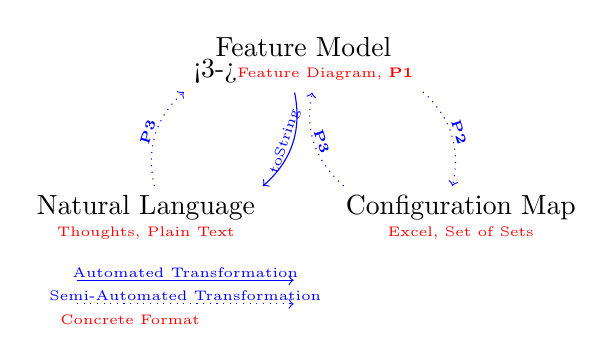
\begin{tikzpicture}
			\tikzstyle{every edge}=[font=\tiny,draw,color=blue]
			\node (fd) at (2,0) [align=center] {Feature Model\\[-1ex]{\uncover<3->{\tiny\color{red}Feature Diagram, \textbf{P1}}}};
			\node (nat) at (0,-2) [align=center] {Natural Language\\[-1ex]{\tiny\color{red}Thoughts, Plain Text}};
			\node (cfg) at (4,-2) [align=center] {Configuration Map\\[-1ex]{\tiny\color{red}Excel, Set of Sets}};

			\path [->] (fd) edge[bend left] node[sloped,yshift=1mm] {toString} (nat);
			\uncover<5->{\path [dotted, ->] (nat) edge[bend left] node[sloped,yshift=1mm] {\textbf{P3}} (fd);}
			
			\uncover<4->{\path [dotted, ->] (fd) edge[bend left] node[sloped,yshift=1mm] {\textbf{P2}} (cfg);}
			\uncover<5->{\path [dotted, ->] (cfg) edge[bend left] node[sloped,yshift=1mm] {\textbf{P3}} (fd);}

			\node (trans) at (-1,-2.8) {};
			\node (trans2) at (2,-2.8) {};
			\node (trans3) at (-1,-3.1) {};
			\node (trans4) at (2,-3.1) {};
			\path [->] (trans) edge node[yshift=1mm] {Automated Transformation} (trans2);
			\path [dotted, ->] (trans3) edge[yshift=5mm] node[yshift=1mm] {Semi-Automated Transformation} (trans4);
		
			\node (bottomleft2) at (-0.2,-3.3) {\tiny\color{red}Concrete Format};
		\end{tikzpicture} % TODO why is feature model to configuration map considered semi-automatically?

		\mynote{Problems}{
			\begin{enumerate}
				\item<3->[P1] How to express feature models \emph{textually}?
				\item<4->[P2] How to (a) validate configurations and (b) get all valid configurations \emph{automatically}?
				\item<5->[P3] \color{gray}{(How to reverse engineer feature models?)}
			\end{enumerate}
		}
	\end{mycolumns}
\end{frame}
% TODO this diagram shows plenty of opportunities for exercise tasks

\subsection{UVL, the Universal Variability Language}

\begin{frame}[fragile]{\myframetitle\ \mytitlesource{\uvlwebsite}}
	\begin{mycolumns}
\begin{uvltight}[basicstyle=\normalsize]{}
features
	ConfigDB
		mandatory
			API {abstract}
				or
					Get
					Put
					Delete

		optional
			Transactions
		mandatory
			OS {abstract}
				alternative
					Windows
					Linux

constraints
	Transactions => Put | Delete
\end{uvltight}
	\mynextcolumn
		\myexampletight{A Feature Model ``Sideways''}{
			\centering
			\pic[width=\linewidth]{varied-model}
			$Transactions \pimplies Put \por Delete$
		}
		\mynote{Universal Variability Language (UVL)}{
			\begin{itemize}
				\item textual language for feature modeling
				\item adds advanced modeling constructs (e.g.,~attributes, cardinalities, submodels, \ldots)
			\end{itemize}
		}
	\end{mycolumns}
\end{frame}

\begin{frame}{Representations and Transformations}
	\begin{mycolumns}
		\centering
		\sffamily
		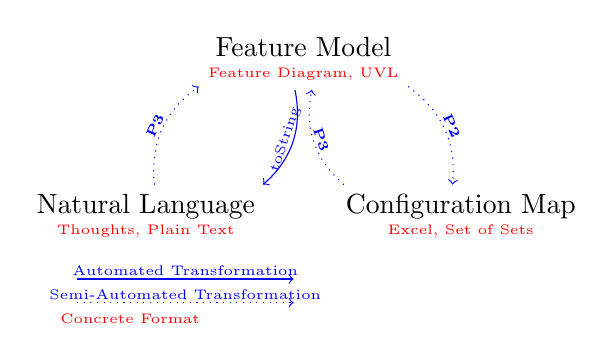
\begin{tikzpicture}
			\tikzstyle{every edge}=[font=\tiny,draw,color=blue]
			\node (fd) at (2,0) [align=center] {Feature Model\\[-1ex]{\tiny\color{red}Feature Diagram, UVL}};
			\node (nat) at (0,-2) [align=center] {Natural Language\\[-1ex]{\tiny\color{red}Thoughts, Plain Text}};
			\node (cfg) at (4,-2) [align=center] {Configuration Map\\[-1ex]{\tiny\color{red}Excel, Set of Sets}};

			\path [->] (fd) edge[bend left] node[sloped,yshift=1mm] {toString} (nat);
			\path [dotted, ->] (nat) edge[bend left] node[sloped,yshift=1mm] {\textbf{P3}} (fd);
			
			\path [dotted, ->] (fd) edge[bend left] node[sloped,yshift=1mm] {\textbf{P2}} (cfg);
			\path [dotted, ->] (cfg) edge[bend left] node[sloped,yshift=1mm] {\textbf{P3}} (fd);

			\node (trans) at (-1,-2.8) {};
			\node (trans2) at (2,-2.8) {};
			\node (trans3) at (-1,-3.1) {};
			\node (trans4) at (2,-3.1) {};
			\path [->] (trans) edge node[yshift=1mm] {Automated Transformation} (trans2);
			\path [dotted, ->] (trans3) edge[yshift=5mm] node[yshift=1mm] {Semi-Automated Transformation} (trans4);
		
			\node (bottomleft2) at (-0.2,-3.3) {\tiny\color{red}Concrete Format};
		\end{tikzpicture}
	\mynextcolumn
		\mynote{Problems}{
			\begin{enumerate}
				\item[P1] How to express feature models \emph{textually}?
				\item[P2] How to (a) validate configurations and (b) get all valid configurations \emph{automatically}?
				\item[P3] \color{gray}{(How to reverse engineer feature models?)}
			\end{enumerate}
		}
		\mynote{Solutions}{
			\begin{enumerate}
				\item[P1] Universal Variability Language $\Rightarrow$ \emph{Syntax}
				\item[P2] \emph{Semantics}?
				\item[P3] \color{gray}{--}
			\end{enumerate}
		}
	\end{mycolumns}
\end{frame}
% TODO do we really need this slide? semantics was already defined in Part 4a for feature models

\subsection{Propositional Formulas}

\subsubsection*{Recap}

\begin{frame}{\myframetitle}
	\begin{mycolumns}
		\mydefinition{Syntax of Propositional Formulas}{
			Inductive definition of \emph{propositional formulas}\\\deutsch{aussagenlogische Formeln}:
			\begin{itemize}
				\item the \emph{Boolean truth values} $\top$, $\bot$
				\item any \emph{Boolean variable} $X$
    			\item any \emph{negation} $\pnot \phi$ of a formula $\phi$
    			\item any \emph{conjunction} $(\phi \pand \psi)$ of formulas $\phi$ and $\psi$
				\item any \emph{disjunction} $(\phi \por \psi)$, \emph{implication} $(\phi \pimplies \psi)$, or \emph{biimplication} $(\phi \pequals \psi)$
			\end{itemize}
		}
	\mynextcolumn
		\mydefinition{Informal Semantics of Propositional Formulas}{
			\vspace*{-4ex}
			\begin{equation*}
				\begin{rcases}
					\top                \\
					\bot                \\
					\pnot \phi          \\
					\phi \pand \psi     \\
					\phi \por \psi      \\
					\phi \pimplies \psi \\
					\phi \pequals \psi
				\end{rcases} \text{ means } \begin{cases}
					\text{``true'' (or \emph{tautology})} \\
					\text{``false'' (or \emph{contradiction})} \\
					\text{``not $\phi$''} \\
					\text{``$\phi$ and $\psi$''} \\
					\text{``$\phi$ or $\psi$'' (inclusive or!)} \\
					\text{``if $\phi$, then $\psi$'' (and else?)} \\
					\text{``$\phi$ if and only if $\psi$''}
				\end{cases}
			\end{equation*}
		}
		\myexample{Operator Precedence: $\pnot$, $\pand$, $\por$, $\pimplies$, $\pequals$}{
			\vspace*{-4ex} % TODO Benno: why is this hack needed?
			\begin{align*}
				           &~Transactions \pimplies (Put \por Delete) \\
				\equiv     &~Transactions \pimplies Put \por Delete \\
				\not\equiv &~(Transactions \pimplies Put) \por Delete
			\end{align*}
		}
% TODO removed this part as we only need propositional logic anyway
%		\mynote{Differences to First-Order Logic}{
%			\begin{itemize}
%				\item no quantifiers $\forall, \exists$
%    			\item no predicates $P(\ldots)$ (e.g., $=$, $>$, $isA$)
%    			\item no functions $f(\ldots)$ (e.g., $+$, $\ast$, $typeOf$)
%				\item no constants (e.g., $42$, ``hello'')
%			\end{itemize}
%		}
	\end{mycolumns}
\end{frame}

\subsubsection*{Example}

\begin{frame}{\myframetitle}
	\begin{mycolumns}[animation=none]
		\only<1-|handout:1-2>{
			\myexampletight{A Feature Model $FM$ \ldots}{
				\centering\tiny
				\featureDiagramConfigurableDatabase[_phi]
				\featureDiagramOverlay{
					\only<1|handout:0>{
						\featureDeemph{(API_phi),(Get_phi),(Put_phi),(Delete_phi),(Transactions_phi),(OS_phi),(Windows_phi),(Linux_phi)}
						\featureEmph{(ConfigDB_phi)}
					}
					\only<2|handout:0>{
						\featureDeemph{(Get_phi),(Put_phi),(Delete_phi),(Transactions_phi),(OS_phi),(Windows_phi),(Linux_phi)}
						\featureEmph{(ConfigDB_phi)(API_phi)}
					}
					\only<3|handout:0>{
						\featureDeemph{(Get_phi),(Put_phi),(Delete_phi),(API_phi),(OS_phi),(Windows_phi),(Linux_phi)}
						\featureEmph{(ConfigDB_phi)(Transactions_phi)}
					}
					\only<4|handout:0>{
						\featureDeemph{(Get_phi),(Put_phi),(Delete_phi),(API_phi),(Transactions_phi),(Windows_phi),(Linux_phi)}
						\featureEmph{(ConfigDB_phi)(OS_phi)}
					}
					\only<5|handout:0>{
						\featureDeemph{(ConfigDB_phi),(Transactions_phi),(Windows_phi),(Linux_phi),(OS_phi)}
						\featureEmph{(Get_phi)(Put_phi)(Delete_phi)(API_phi)}
					}
					\only<6-7|handout:0>{
						\featureDeemph{(Get_phi),(Put_phi),(Delete_phi),(API_phi),(Transactions_phi),(ConfigDB_phi)}
						\featureEmph{(Windows_phi)(Linux_phi)(OS_phi)}
					}
					\only<8|handout:0>{
						\featureDeemph{(ConfigDB_phi)(Transactions_phi)(Windows_phi)(Linux_phi)(OS_phi)(Get_phi)(Put_phi)(Delete_phi)(API_phi)}
					}
					\only<9-12|handout:1>{
						\featureSelected{(ConfigDB_phi),(API_phi),(Get_phi),(OS_phi),(Windows_phi)}
						\featureDeselected{(Put_phi)(Delete_phi),(Transactions_phi),(Linux_phi)}
					}
					\only<13-|handout:2>{
						\featureSelected{(ConfigDB_phi),(API_phi),(Get_phi)}
						\featureDeselected{(Put_phi)(Delete_phi)(Windows_phi)(Linux_phi),(Transactions_phi)(OS_phi)}
					}
				}
			}
			\myexample{\ldots as a Propositional Formula $\Phi(FM)$}{
				\vspace*{-4ex}
				\small
				\begin{align*}
					\Phi(FM) = &~ConfigDB \\
					\uncover<2->{\pand &~(API \pequals ConfigDB) \\}
					\uncover<3->{\pand &~(Transactions \pimplies ConfigDB) \\}
					\uncover<4->{\pand &~(OS \pequals ConfigDB) \\}
					\uncover<5->{\pand &~(Get \por Put \por Delete \pequals API) \\}
					\uncover<6->{\pand &~(Windows \por Linux \pequals OS) \\}
					\uncover<7->{\pand &~\pnot (Windows \pand Linux) \\}
					\uncover<8->{\pand &~(Transactions \pimplies Put \por Delete)}
				\end{align*}
			}
		}
	\mynextcolumn
		\only<9-|handout:1-2>{
			\myexample{Is This a Valid Configuration?}{
				\vspace*{-4ex}
				\only<9-12|handout:1>{
					\begin{align*}
								&~\Phi(FM)({\{C, A, G, O, W\}}) \\
						\equiv	&~\Phi(FM)(\cfg[2-]{C, A, G, O, W}{P, D, T, L}) \\
						\uncover<10->{\equiv &~\fs{C} \pand (\fs{A} \pequals \fs{C}) \pand (\fd{T} \pimplies \fs{C}) \pand (\fs{O} \pequals \fs{C}) \\
								&~\pand (\fs{G} \por \fd{P} \por \fd{D} \pequals \fs{A}) \pand (\fs{W} \por \fd{L} \pequals \fs{O}) \\
								&~\pand \pnot (\fs{W} \pand \fd{L}) \pand (\fd{T} \pimplies \fd{P} \por \fd{D}) \\}
						\uncover<11->{\equiv &~\fs{\top} \pand (\fs{\top} \pequals \fs{\top}) \pand (\fd{\bot} \pimplies \fs{\top}) \pand (\fs{\top} \pequals \fs{\top}) \\
								&~\pand (\fs{\top} \por \fd{\bot} \por \fd{\bot} \pequals \fs{\top}) \pand (\fs{\top} \por \fd{\bot} \pequals \fs{\top}) \\
								&~\pand \pnot (\fs{\top} \pand \fd{\bot}) \pand (\fd{\bot} \pimplies \fd{\bot} \por \fd{\bot}) \\}
						\uncover<12->{\equiv &~\fs{\top} \pand \fs{\top} \pand \fs{\top} \pand \fs{\top} \pand \fs{\top} \pand \fs{\top} \pand \fs{\top} \pand \fs{\top} \\
						\equiv	&~\fs{\top}}
					\end{align*}
					\uncover<12->{\emph{$\leadsto$ configuration is valid}\\
					\phantom{$\leadsto$ }(read-only database on Windows)}
				}
				\only<13-|handout:2>{
					\begin{align*}
								&~\Phi(FM)({\{C, A, G\}}) \\
						\equiv	&~\Phi(FM)(\cfg[2-]{C, A, G}{P, D, T, O, W, L}) \\
						\uncover<14->{\equiv&~\fs{C} \pand (\fs{A} \pequals \fs{C}) \pand (\fd{T} \pimplies \fs{C}) \pand (\fd{O} \pequals \fs{C}) \\
								&~\pand (\fs{G} \por \fd{P} \por \fd{D} \pequals \fs{A}) \pand (\fd{W} \por \fd{L} \pequals \fd{O}) \\
								&~\pand \pnot (\fd{W} \pand \fd{L}) \pand (\fd{T} \pimplies \fd{P} \por \fd{D}) \\}
						\uncover<15->{\equiv&~\fs{\top} \pand (\fs{\top} \pequals \fs{\top}) \pand (\fd{\bot} \pimplies \fs{\top}) \pand (\fd{\bot} \pequals \fs{\top}) \\
								&~\pand (\fs{\top} \por \fd{\bot} \por \fd{\bot} \pequals \fs{\top}) \pand (\fd{\bot} \por \fd{\bot} \pequals \fd{\bot}) \\
								&~\pand \pnot (\fd{\bot} \pand \fd{\bot}) \pand (\fd{\bot} \pimplies \fd{\bot} \por \fd{\bot}) \\}
						\uncover<16->{\equiv&~\fs{\top} \pand \fs{\top} \pand \fs{\top} \pand \fd{\bot} \pand \fs{\top} \pand \fs{\top} \pand \fs{\top} \pand \fs{\top} \\
						\equiv	&~\fd{\bot}} % TODO: only show \pand and phi(fm) = and parentheses at the end
					\end{align*}
					\uncover<16->{\emph{$\leadsto$ configuration is invalid}\\
					\phantom{$\leadsto$ }($\lightning$ no operating system)}
				}
			}
		}
	\end{mycolumns}
\end{frame}

\subsubsection*{Algorithm}

\newcommand{\featureDiagramFn}[4]{#1\left(~\parbox{#2}{\centering\scalebox{0.8}{\featureDiagram{#3}}}~\right) &= #4}
\newcommand{\featureDiagramPhantom}[4]{\vphantom{#1\left(~\parbox{#2}{\centering\scalebox{0.8}{\featureDiagram{#3}}}~\right)}}

\begin{frame}{\myframetitle}
	\begin{mycolumns}[animation=none]
		\mydefinition{Algorithm: Translate $FM$ Into $\Phi(FM)$}{
			\begin{enumerate}
				\item<2-> translate each tree constraint
				\begin{itemize}
					\item<3-> \emph{Root feature}: $R$ is always required
						\item<4-> \emph{Optional feature}: $C$ requires $P$
						\item<5-> \emph{Mandatory feature}:\\
							Optional + $P$ requires $C$
						\item<6-> \emph{Or group}:\\
							Optional + $P$ requires at least one $C_i$
						\item<7-> \emph{Alternative group}:\\
							Optional + $P$ requires exactly one $C_i$
				\end{itemize}
				\item<8-> conjoin translated tree constraints\\
					$\Phi(TC) \gets \bigwedge_{tc \in TC} \Phi(tc)$
				\item<9-> conjoin \emph{cross-tree constraints}\\
					$\Phi(CTC) \gets \bigwedge_{ctc \in CTC} ctc$
				\item<10-> $\Phi(FM) \gets \Phi(TC) \pand \Phi(CTC)$
			\end{enumerate}
		}
	\mynextcolumn
		\mydefinition{}{
			\vspace*{-4ex}
			\begin{align*}
				\uncover<3->{\featureDiagramFn{\Phi}{6ex}{Root,concrete}{Root}}\\
				\uncover<4->{\featureDiagramFn{\Phi}{6ex}{P,concrete[C,optional,concrete]}{C \pimplies P}}\\
				\uncover<5->{\featureDiagramFn{\Phi}{6ex}{P,concrete[C,mandatory,concrete]}{C \pequals P}}\\
				\uncover<6->{\featureDiagramFn{\Phi}{15ex}{P,concrete[$C_1$,or,concrete][\ldots,concrete][$C_n$,concrete]}{\bigvee_{1 \leq i \leq n} C_i \pequals P}}\\
				\uncover<7->{\featureDiagramFn{\Phi}{15ex}{P,concrete[$C_1$,alternative,concrete][\ldots,concrete][$C_n$,concrete]}{\bigvee_{1 \leq i \leq n} C_i \pequals P}}\\
				\uncover<7->{& \pand \bigwedge_{1 \leq i < j \leq n} \pnot (C_i \pand C_j)}
			\end{align*}
		}
	\end{mycolumns}
\end{frame}

\subsection{CNF as a Universal Formula Language}

\begin{frame}{\myframetitle} % TODO unmotivated topic switch after prior slide?
	\begin{mycolumns}[animation=none]
		\mydefinition{Recap: Conjunctive Normal Form}{
			\begin{itemize}
				\item a \emph{literal} $L$ is a variable $X$ or its negation $\pnot X$
				\item a \emph{clause} $\clause{C}$ is a disjunction of literals $\clause{\bigvee_{j} L_j}$
				\item a \emph{conjunctive normal form (CNF)} is a conjunction of clauses $\bigwedge_{i} \clause{C_i} = \bigwedge_{i} \clause{\bigvee_{j} L_j}$
				\item intuitively: a set of ``rules'' to be satisfied
				\item any formula $\phi$ can be transformed into a CNF $\phi'$ that is logically equivalent ($\phi \mequals \phi'$)
			\end{itemize}
		}
		\uncover<2->{
			\mydefinition{Recap: Laws of Propositional Logic}{
				\begin{itemize}
					\item<3-> implication: $\phi \pimplies \psi \mequals \pnot \phi \por \psi$
					\item<3-> biimplication: $\phi \pequals \psi \mequals (\pnot \phi \por \psi) \pand (\pnot \psi \por \phi)$
					\item<4-> De Morgan's laws: $\pnot (\phi \pand \psi) \mequals \pnot \phi \por \pnot \psi$
					\item<5-> distributivity:\,$(\phi \pand \psi) \por \chi \mequals (\phi \por \chi) \pand (\psi \por \chi)$
				\end{itemize}
			}
		}
	\mynextcolumn
		\uncover<2->{
			\myexample{Transforming Part of $\Phi(FM)$ into $CNF(\Phi(FM))$}{
				\vspace*{-4ex}
				\small
				% TODO: use color-blind friendly colors
				\leftandright{
					\begin{align*}
						\uncover<2->{&~\clause{C} \\
						\pand &~(T \pimplies C) \\
						\pand &~(O \pequals C) \\
						\pand &~(W \por L \pequals O) \\
						\pand &~\pnot (W \pand L)}
					\end{align*}
				}{
					\begin{align*}
						\uncover<3->{&~\clause{C} \\
						\pand &~\clause{(\pnot T \por C)} \\
						\pand &~\clause{(\pnot O \por C)} \pand \clause{(\pnot C \por O)} \\
						\pand &~(\pnot (W \por L) \por O) \\
						\pand &~\clause{(\pnot O \por W \por L)} \\
						\pand &~\pnot (W \pand L)}
					\end{align*}
				}
				\leftandright{
					\begin{align*}
						\uncover<4->{&~\clause{C} \\
						\pand &~\clause{(\pnot T \por C)} \\
						\pand &~\clause{(\pnot O \por C)} \pand \clause{(\pnot C \por O)} \\
						\pand &~((\pnot W \pand \pnot L) \por O) \\
						\pand &~\clause{(\pnot O \por W \por L)} \\
						\pand &~\clause{(\pnot W \por \pnot L)}}
					\end{align*}
				}{
					\begin{align*}
						\uncover<5->{&~\clause{C} \\
						\pand &~\clause{(\pnot T \por C)} \\
						\pand &~\clause{(\pnot O \por C)} \pand \clause{(\pnot C \por O)} \\
						\pand &~\clause{(\pnot W \por O)} \pand \clause{(\pnot L \por O)} \\
						\pand &~\clause{(\pnot O \por W \por L)} \\
						\pand &~\clause{(\pnot W \por \pnot L)}}
					\end{align*}
				}
			}
		}
	\end{mycolumns}
\end{frame} % TODO would be more intuitive to me if clauses are green (as they are good to go)

\subsubsection*{DIMACS}

\begin{frame}[fragile]{\myframetitle}
 	\begin{mycolumns}[columns=3,widths={25,25,50}]
		\vspace*{14ex}
		\begin{align*}
			&~C \\
			\pand &~(\pnot T \por C) \\
			\pand &~(\pnot O \por C) \pand (\pnot C \por O) \\
			\pand &~(\pnot W \por O) \pand (\pnot L \por O) \\
			\pand &~(\pnot O \por W \por L) \\
			\pand &~(\pnot W \por \pnot L)
		\end{align*}
 	\mynextcolumn
\begin{dimacstight}[basicstyle=\large]{}
c 1 C
c 2 T
c 3 O
c 4 W
c 5 L
p cnf 5 6
1 0
-2 1 0
-3 1 0 -1 3 0
-4 3 0 -5 3 0
-3 4 5 0
-4 5 0
\end{dimacstight}
	\mynextcolumn
		\mydefinition{DIMACS Format\mysource{\dimacsformat}}{
			\begin{itemize}
				\item de facto industry standard for storing CNF
				\item machine-readable, automated analyses, \ldots
				\item comments start with \texttt{c \ldots}
				\item problem line:\\
					\texttt{p cnf \#variables \#clauses}
				\item clause $\bigvee_{i} L_i$ translates to \texttt{L1 \ldots\ Ln 0}
				\item intuitively:
					\begin{equation*}
						\begin{rcases}
							\texttt{0}\\
							\texttt{\textvisiblespace}\\
							\texttt{-}
						\end{rcases} \text{ means } \begin{cases}
							\pand \\
							\por \\
							\pnot
						\end{cases}
					\end{equation*}
			\end{itemize}
		}
 	\end{mycolumns}
\end{frame}

\begin{frame}{Representations and Transformations}
	\begin{mycolumns}[widths={52,48}]
		\centering
		\sffamily
		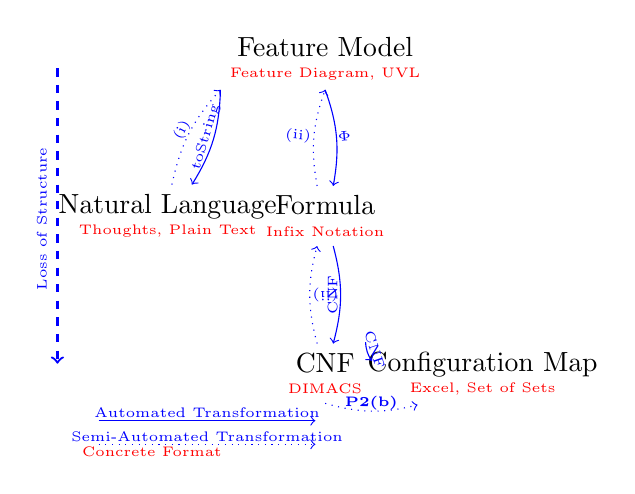
\begin{tikzpicture}
			\tikzstyle{every edge}=[font=\tiny,draw,color=blue]

			\node (topleft) at (-1.4,0) {};
			\node (bottomleft) at (-1.4,-4) {};
			
			\node (fd) at (2,0) [align=center] {Feature Model\\[-1ex]{\tiny\color{red}Feature Diagram, UVL}};
			\node (nat) at (0,-2) [align=center] {Natural Language\\[-1ex]{\tiny\color{red}Thoughts, Plain Text}};
			\node (phi) at (2,-2) [align=center] {Formula\\[-1ex]{\tiny\color{red}Infix Notation}};
			\node (cfg) at (4,-4) [align=center] {Configuration Map\\[-1ex]{\tiny\color{red}Excel, Set of Sets}};
			\node (cnf) at (2,-4) [align=center] {CNF\\[-1ex]{\tiny\color{red}DIMACS}};

			\path [dashed, thick, ->] (topleft) edge node[left, rotate=90, yshift=2mm, xshift=10mm] {Loss of Structure} (bottomleft);
		
			\path [->] (fd.south west) edge[bend left=15] node[sloped,yshift=1mm] {toString} (nat);
			\path [dotted, ->] (nat) edge[bend left=15] node[sloped,yshift=1mm] {(i)} (fd.south west);
			
			\path [->] (fd.south) edge[bend left=15] node[sloped,yshift=1mm,rotate=90] {$\Phi$} (phi);
			\path [dotted, ->] (phi) edge[bend left=15] node[sloped,yshift=2mm,rotate=270] {(ii)} (fd.south);

			\path [->] (phi) edge[bend left=15] node[sloped,yshift=1mm] {CNF} (cnf);
			\path [dotted, ->] (cnf) edge[bend left=15] node[sloped,yshift=2mm,rotate=270] {(ii)} (phi);
		
			\path [->] (cfg) edge[bend right=15] node[sloped,yshift=1mm] {CNF} (cnf);
			\path [dotted, ->] (cnf.south) edge[bend right=15] node[sloped,yshift=1mm] {\textbf{P2(b)}} (cfg);

			\node (trans) at (-1,-4.6) {};
			\node (trans2) at (2,-4.6) {};
			\node (trans3) at (-1,-4.9) {};
			\node (trans4) at (2,-4.9) {};
			\path [->] (trans) edge node[yshift=1mm] {Automated Transformation} (trans2);
			\path [dotted, ->] (trans3) edge[yshift=5mm] node[yshift=1mm] {Semi-Automated Transformation} (trans4);
		
			\node (bottomleft2) at (-0.2,-5) {\tiny\color{red}Concrete Format};
		\end{tikzpicture} % TODO would prefer another color for concrete formats, as they have nothing to do with the red boxes on thoses slides. what about green? needs to be changed consistently in all slides of this lecture
	\mynextcolumn
		\mynote{Problems}{
			\begin{enumerate}
				\item[P1] How to express feature models \emph{textually}?
				\item[P2] How to 
				\begin{itemize}
					\item[(a)] validate configurations and
					\item[(b)] get all valid configurations
				\end{itemize}
				\emph{automatically}?
				\item[P3] \color{gray}{(How to reverse engineer feature models?)}
			\end{enumerate}
		}
		\mynote{Solutions}{
			\begin{enumerate}
				\item[P1] Universal Variability Language $\Rightarrow$ \emph{Syntax}
				\item[P2] Propositional Formulas $\Rightarrow$ \emph{Semantics}
				\begin{itemize}
					\item[(a)] evaluate feature-model formula
					\item[(b)] \emph{???}
				\end{itemize}
				\item[P3] \color{gray}{(i) e.g., \bakarnaturallanguage\\(ii) e.g., \czarneckithereandbackagain}
			\end{enumerate}
		}
	\end{mycolumns}
\end{frame}

\subsection{Feature Models in the Wild}

\subsubsection*{Excel, Again}

\begin{frame}{\myframetitle}
	\centering
	\pic[width=.8\linewidth,trim=10 10 0 10,clip]{constraints-in-excel}

	\textbf{``It's installed anyway.''}
\end{frame}

\subsubsection*{Linux Kernel}

\begin{frame}[fragile]{\myframetitle}
	\begin{mycolumns}
		\begin{kconfigtight}[basicstyle=\small]{Part of the x86 Architecture \mysource{\href{https://github.com/torvalds/linux/blob/0326074/arch/x86/Kconfig}{linux/arch/x86/Kconfig}}}
config 64BIT
	bool "64-bit kernel" if "$(ARCH)" = "x86"
	default "$(ARCH)" != "i386"
	help
		Say yes to build a 64-bit kernel (x86_64)
		Say no to build a 32-bit kernel (i386)

config X86_32
	def_bool y
	depends on !64BIT
	# Options that are inherently 32-bit kernel only:
	select GENERIC_VDSO_32
	select ARCH_SPLIT_ARG64

config X86_64
	def_bool y
	depends on 64BIT
	# Options that are inherently 64-bit kernel only:
	select ARCH_HAS_GIGANTIC_PAGE
	select ARCH_SUPPORTS_INT128 if CC_HAS_INT128
\end{kconfigtight}
	\mynextcolumn
		\mydefinition{KConfig Language\mysource{\href{https://www.kernel.org/doc/html/latest/kbuild/kconfig-language.html}{kernel.org}}}{
			\begin{itemize}
				\item configuration language used in embedded/OS development (e.g., Linux, Zephyr, ESP32)
				\item similar to UVL, but has many quirks (e.g., tristate features, \texttt{select})
				\item transformation into formula or feature model possible, but not trivial \mysource{\href{https://dl.acm.org/doi/abs/10.1145/3468264.3468578}{Oh~et~al.~2021}}
			\end{itemize}
		}
		\hspace*{-0.07253886\linewidth}%=2*0.035/(1-0.035)
		\linuxbddlink{\includegraphics[width=1.3\linewidth,trim=220 510 60 180,clip]{2020/2020-SPLC-Thuem}}
	\end{mycolumns}
\end{frame}